\chapter{Medición de los poros de la lámina cribosa}
\section{Problema}
En el curso de la investigación que se está llevando a cabo
actualmente sobre el \emph{\gls{glaucoma}} y las causas que lo
provocan, se ha detectado una posible relación con la aparición y
tamaño de los poros de la \emph{\gls{lamina-cribosa}} en la
\emph{\gls{papila-optica}} o cabeza del nervio óptico. \\
La \emph{\gls{papila-optica}} o \emph{disco óptico} es el punto donde
el nervio óptico entra en el globo ocular. Tiene la forma de un
pequeño disco rosado de aproximadamente $2 \times 1.5$ milímetros y
está situado en la parte posterior del globo ocular. Hasta hace
relativamente poco no se sabía mucho de ella debido a las carencias
tecnológicas. Gracias a las \gls{tco}, se han podido conseguir datos
con cierta precisión, entre los que se encuentra el objeto de este
estudio: unos poros de los que se cree que puedan estar
relacionados con la evolución del \emph{\gls{glaucoma}}.

\section{Objetivos}
El objetivo principal de esta parte de la investigación implica
encontrar automáticamente, mediante algoritmos de visión
computarizada, los poros del disco óptico para medirlos y, en la
medida de lo posible, establecer una correlación entre su tamaño, la
cantidad, la posición o la forma y el estado evolutivo del
\emph{\gls{glaucoma}}, siendo este procedimiento supervisado por
personal médico.
\begin{itemize}
\item Detección de los poros de la papila así como también de la mayor
  cantidad posible de sus propiedades: área, coordenadas,
  distribución, etc.
\end{itemize}

\section{Estudio}
Al ser un estudio pionero, lo primero que se procedió a realizar fue
un análisis previo de viabilidad de las \gls{tco} obtenidas. El
principal problema encontrado es la dificultad de enfoque de la papila
que provoca que las imágenes sean totalmente distintas por cada
paciente debido a que no todos los pacientes toleran de igual manera
el tiempo de exposición durante el proceso de exploración. Sin
embargo, con el enfoque adecuado, sí es viable proceder a estudiar los
poros, aunque no se ha encontrado todavía una forma clara de
estandarizar el proceso a todos los pacientes hasta que se consiga
reducir el tiempo de exploración. Una vez demostrado la viabilidad de
las \gls{tco} que produce la máquina, se procedió a
realizar el estudio.\\
Los dos problemas principales, a pesar de todas las técnicas y tiempo
dedicados en su solución, son la dificultad de enfoque de los poros y
su profundidad visible en la \gls{tco} lo que provoca desconocimiento
en la reducción de detección de falsos poros mediante la aplicación,
de manera genérica, de algoritmos de búsqueda de zonas de
interés\deftecnica{tecnica:blobs}. Aún así, se tuvo muy en cuenta
durante todo el proceso la utilización y el análisis de resultados del
algoritmo \emph{\gls{ORB}~\citep*{orb-bib}}
\begin{enumerate}
\item Se realiza una búsqueda de los poros mediante la técnica
  \emph{findBlobs} de \emph{SimpleCV} con área máxima de $150$
  píxeles. Este área máximo se determinó tras realizar pruebas
  y comprobar que los poros más grandes encontrados en los casos
  de mayor deterioro no superan este tamaño. De esta forma se
  descartan \emph{blobs} detectados por el algoritmo que no son 
  poros reales.
\end{enumerate}

\section{Algoritmo propuesto}
Esta sección se deja vacía por la ausencia de una propuesta propia
debido a la imposibilidad explicada en la sección anterior de mejorar
las ya existentes técnicas. Sin embargo, se proporciona descrito en
profundidad el código concreto de la biblioteca usada para tal efecto.

\begin{figure}[H]
  \caption{Detección de poros}
  \centering \setlength\fboxsep{0pt} \setlength\fboxrule{0.5pt}
  \fbox{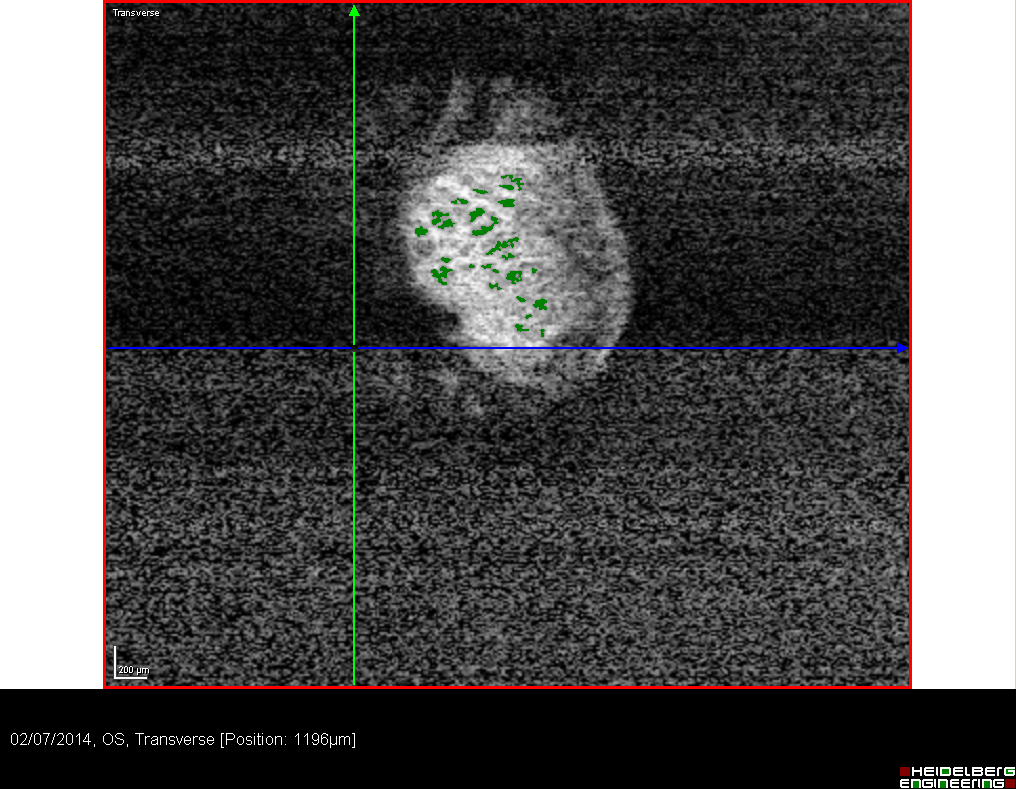
\includegraphics[width=\textwidth]{imagenes/poros_papila/porosPapila.png}}
    \end{figure}